%%%%%%%%%%%%%%%%%%%%%%% file template.tex %%%%%%%%%%%%%%%%%%%%%%%%%
%
% This is a general template file for the LaTeX package SVJour3
% for Springer journals.          Springer Heidelberg 2010/09/16
%
% Copy it to a new file with a new name and use it as the basis
% for your article. Delete % signs as needed.
%
% This template includes a few options for different layouts and
% content for various journals. Please consult a previous issue of
% your journal as needed.
%
%
\RequirePackage{fix-cm}
%
\documentclass{svjour3}                     % onecolumn (standard format)
%\documentclass[smallcondensed]{svjour3}     % onecolumn (ditto)
%\documentclass[smallextended]{svjour3}       % onecolumn (second format)
%\documentclass[twocolumn]{svjour3}          % twocolumn
%
\smartqed  % flush right qed marks, e.g. at end of proof
%
\usepackage[ruled, vlined, linesnumbered]{algorithm2e}

\usepackage{amsmath,amssymb}
\usepackage{graphicx}
\usepackage{times}
\usepackage{url}
\usepackage{color}
\definecolor{Orange}{rgb}{1,0.5,0}
\newcommand{\todo}[1]{\textsf{\textbf{\textcolor{Orange}{[[#1]]}}}}
%
% \usepackage{mathptmx}      % use Times fonts if available on your TeX system
%
% insert here the call for the packages your document requires
%\usepackage{latexsym}
% etc.
%
% please place your own definitions here and don't use \def but
% \newcommand{}{}
%
% Insert the name of "your journal" with
% \journalname{myjournal}
%
\begin{document}

% In the original styles from ACM, you would have needed to
% add meta-info here. This is not necessary for AAMAS 2014  as
% the complete copyright information is generated by the cls-files.


\title{Human-Agent Collaboration for Disaster Response}

% AUTHORS


% For initial submission, do not give author names, but the
% tracking number, instead, as the review process is blind.

% You need the command \numberofauthors to handle the 'placement
% and alignment' of the authors beneath the title.
%
% For aesthetic reasons, we recommend 'three authors at a time'
% i.e. three 'name/affiliation blocks' be placed beneath the title.
%
% NOTE: You are NOT restricted in how many 'rows' of
% "name/affiliations" may appear. We just ask that you restrict
% the number of 'columns' to three.
%
% Because of the available 'opening page real-estate'
% we ask you to refrain from putting more than six authors
% (two rows with three columns) beneath the article title.
% More than six makes the first-page appear very cluttered indeed.
%
% Use the \alignauthor commands to handle the names
% and affiliations for an 'aesthetic maximum' of six authors.
% Add names, affiliations, addresses for
% the seventh etc. author(s) as the argument for the
% \additionalauthors command.
% These 'additional authors' will be output/set for you
% without further effort on your part as the last section in
% the body of your article BEFORE References or any Appendices.

%\numberofauthors{8} %  in this sample file, there are a *total*
% of EIGHT authors. SIX appear on the 'first-page' (for formatting
% reasons) and the remaining two appear in the \additionalauthors section.
%

% \author{
% You can go ahead and credit any number of authors here,
% e.g. one 'row of three' or two rows (consisting of one row of three
% and a second row of one, two or three).
%
% The command \alignauthor (no curly braces needed) should
% precede each author name, affiliation/snail-mail address and
% e-mail address. Additionally, tag each line of
% affiliation/address with \affaddr, and tag the
% e-mail address with \email.
% 1st. author
\author{XX,YY,ZZ}
\author{Sarvapali D. Ramchurn \and Feng Wu \and Wenchao Jiang \and Joel Fischer \and Steve Reece \and Stephen Roberts \and Tom Rodden \and Chris Greenhalgh \and  Nicholas R. Jennings 
}

%\authorrunning{Short form of author list} % if too long for running head
%

%\institute{XX \at
%              XX\\
%              \email{\{XX\}}           %  \\
%           \and
%           YY \at
%              YY\\
%		\email{\{YY\}}
%\and
%           ZZ \at
%             ZZ\\
%		\email{\{ZZ\}}}

\institute{Sarvapali D. Ramchurn, Feng Wu, and Nick Jennings \at
              Electronics  and Computer Science, 
	    University of Southampton, UK\\
              \email{\{sdr1,fw1e11,nrj\}@soton.ac.uk}           %  \\
           \and
           Wenchao Jiang, Joel Fischer, Chris Greenhalgh, and Tom Rodden \at
              Mixed Reality Lab, 
		University of Nottingham,
		Nottingham, UK\\
		\email{\{psxwj,jef,cmg,tar\}@cs.nott.ac.uk}
\and
           Steve Reece and Stephen Roberts \at
              Pattern Recognition Group, 
		University of Oxford,
		Oxford, UK\\
		\email{\{reece,roberts\}@robots.ox.ac.uk}}

%% There's nothing stopping you putting the seventh, eighth, etc.
%% author on the opening page (as the 'third row') but we ask,
%% for aesthetic reasons that you place these 'additional authors'
%% in the \additional authors block, viz.
%\additionalauthors{Additional authors: John Smith (The Th{\o}rv{\"a}ld Group,
%email: {\texttt{jsmith@affiliation.org}}) and Julius P.~Kumquat
%(The Kumquat Consortium, email: {\texttt{jpkumquat@consortium.net}}).}
%\date{30 July 1999}
%% Just remember to make sure that the TOTAL number of authors
%% is the number that will appear on the first page PLUS the
%% number that will appear in the \additionalauthors section.
\date{Received: date / Accepted: date}
\maketitle

\begin{abstract}
In the aftermath of major disasters, first responders are typically
overwhelmed with large numbers of, spatially distributed, search and
rescue tasks, each with their own requirements. Moreover, responders
have to operate in highly uncertain and dynamic environments where new
tasks may appear and hazards may be spreading across the disaster
space. Hence, rescue missions may need to be re-planned as new
information comes in, tasks are completed, or new hazards are
discovered. Hence, finding an optimal allocation of resources to
complete all the tasks is a major computational challenge. Indeed,  a
number of agent-based solutions have been developed to help human
commanders perform such planning tasks. However, studies have shown
that, unless these solutions minimise the cognitive burden imposed on
human commanders and first responders, they may hinder task
performance rather than help.  It is therefore crucial to deploy such
agent-based planning solutions alongside human commanders in order to
uncover the interactional issues that arise. Hence, in this paper, we
use decision theoretic techniques to solve the task allocation problem
posed by emergency response planning and then deploy our solution as
part of an agent-based planning tool in  real-world field trials. By
so doing, we are able to study the interactional issues that arise
when humans are guided by an agent. In more detail, we develop an
algorithm, based on a  Multi-Agent Markov Decision Process
representation of the task allocation problem and show that it
outperforms standard benchmarks from the literature. We then integrate
the algorithm into a planning agent that responds to requests for
tasks from  participants in a mixed-reality location-based game,
called AtomicOrchid, that simulates disaster response settings in the
real-world.  We then run a number of trials of our planning agent and
compare it against a purely human driven system. Our  analysis of
these trials show that human commanders adapt to the planning agent by
taking on a more supervisory role and that, by providing humans with the flexibility of requesting plans from the agent, allows them to perform more tasks more efficiently than using purely human interactions to allocate tasks. We also discuss how such flexibility could lead to poor performance if left unchecked.  \end{abstract}

% Note that the category section should be completed after reference to the ACM Computing Classification Scheme available at
% http://www.acm.org/about/class/1998/.

\keywords{Human-Agent Interaction, Human-Agent Collectives, Disaster Response.}

\section{Introduction}
\noindent The coordination of first responders in search and rescue missions is a grand challenge for multi-agent systems research \cite{kitano:2001}. In such settings, responders with different capabilities (e.g., fire-fighting or life support) have to form teams in order to perform rescue tasks  (e.g., extinguishing a fire or providing first aid) to minimise  loss of life and costs (e.g., time or money). These tasks may be geographically distributed  and require specific teams  to be completed. Furthermore, uncertainty in the environment (e.g., wind direction or spread of fire) or in the responders' abilities to complete tasks (e.g., some may be tired or get hurt) means that plans are likely to change continually to reflect the prevailing assessment of the situation. 

To address these challenges, a number of algorithms  have been developed to form teams and allocate tasks. For example, \cite{ramchurn:etal:2010,Scerri2005} and \cite{Chapman2009}, devised centralised and decentralised algorithms respectively to allocate rescue tasks to first responders with different capabilities. However, none of these approaches considered the inherent uncertainty in the environment or in the first responders' abilities. Crucially, to date, while all of these algorithms have been shown to perform well in simulations (representing responders as computational entities), none of them have been \emph{trialled} to guide \emph{real} human responders in real-time rescue missions. Thus, it is still unclear whether these algorithms will cope with real-world uncertainties (e.g., social preference), be acceptable to humans (i.e., be intelligible and effective), and actually augment, rather than hinder,  human performance.

Against this background, we develop a novel algorithm for team coordination under uncertainty and evaluate it within a real-world \emph{mixed-reality game} \cite{Fischer:etal:2012} that embodies the simulation of team coordination in disaster response settings. Specifically, our algorithm is used by a software agent to guide human responders in the game to stay clear of a virtual radioactive cloud and complete a number of geo-located rescue tasks in the real world. By so doing, we  study, both quantitatively and qualitatively, the performance of a human-agent collective (i.e., a mixed-initiative team where control can shift between humans and agents)  and the interactions between the different actors in the system. In particular, we  advance the state of the art in the following ways. First, we develop a novel representation for team coordination (i.e., path planning and task allocation) under uncertainty using Multi-agent Markov Decision Processes (MMDP)  \cite{boutilier1996planning}. Moreover, we provide an approximate algorithm to solve the MMDP and show how it  is adaptive to human requests to re-plan task allocations. Second, we present AtomicOrchid, a novel game to evaluate team coordination under uncertainty using the concept of mixed-reality games. AtomicOrchid allows a planning agent, using our task planning algorithm, to coordinate, in real-time, human players using mobile phone-based messaging, to complete rescue tasks efficiently. Third, we provide a real-world evaluation of our planning agent in a disaster response scenario in multiple field trials and present both quantitative and qualitative results. 
Our results show, for the first time, how agent-based coordination algorithms for disaster response can be integrated and validated with human teams. Moreover, these results allow us to derive  guidelines for systems involving  human-agent collaboration.  In what follows, we first formalise the disaster response problem as a MMDP and then describe the algorithms to solve the the MMDP. Given this we describe the AtomicOrchid platform and present results of our field trials and discuss our design guidelines for human-agent collaboration.\vspace{-2mm}


%%%%%%%%%%%%%%%%%%%%%%%%%%% OLD TEXT %%%%%%%%%%%%%%%%%%%%%%%%%%%%

%In more detail, we consider a scenario involving rescue tasks distributed in a physical space over which a (virtual) radioactive cloud is spreading. Tasks need to be completed by the responders before the area is completely covered by the cloud (as responders will die from radiation exposure) which is spreading according to varying wind speed and direction. Our algorithm captures the uncertainty in the scenario (i.e., in terms of environment and player states) and  is able to compute a policy to allocate responders to tasks that minimises task completion time and ensures responders are not exposed to significant radiation. The algorithm is then used by an agent to guide human responders. Specifically


%The rest of this paper is structured as follows. First we \ref{sec:scenario} formalises the disaster response problem as a MMDP. Section \ref{sec:algo}  describes the algorithms to solve the the MMDP while Section \ref{sec:atomicorchid}  details the AtomicOrchid platform. Section \ref{sec:evaluation} presents our field trials and Section \ref{sec:conclusions} concludes.
\section{Background}
\todo{Background on
\begin{enumerate}
\item Gopal's background on coordination for disaster response, RoboCup Rescue, and Scerri's work.
\item Feng's background on MDP approaches to coordination (incl CFST and Archie's paper)
\item Joel/Wenchao to add background on HCI studies on coordination in disasters + mixed reality 
\end{enumerate}}
\todo{
The following are a few suggestions for improving the work.
-- the paper should cite the work by Humphereys and Adams that discussed assignment of responders in emergency situations. Their work is particularly relevant because of the way they balanced competing task demands.
}

\todo{Please add more references to cover beyond what we do to some extent}
\section{The Disaster Scenario}

\noindent We consider a disaster scenario involving a satellite, powered radioactive fuel, that has crashed in a sub-urban area (see Section \ref{atomic} to see how this helps implement a  mixed-reality game). While debris is strewn around a large area, damaging buildings and causing accidents and injuring civilians, radioactive particles discharged in the air, from the debris, are gradually spreading over the area, threatening to contaminate food reserves and people. Hence, emergency services, voluntary organisations, and the military are deployed to help evacuate the casualties and resources before these are engulfed by  radioactive cloud.  In what follows, we model this scenario formally and then describe the optimisation problem faced by the actors  (i.e., including emergency services, volunteers, medics, and soldiers) in trying to save as many lives and resources as possible.  We then propose an algorithm to solve this optimisation problem (in Section \ref{sec:algo}. In Section \ref{sec:atomic}, we show how this algorithm can be used by a software agent (in our mixed-reality game) in a mixed-initiative process to coordinate field responders. 

\subsection{Formal Model}
\noindent Let $G$ denote a grid overlaid on top of the disaster space, and the satellite and actors are located at various coordinates $(x,y) \in G$ in this grid. The radioactive cloud induces a radioactivity level  $l \in [0,100]$ at every point it covers in the grid (100 corresponds to maximum radiation). While the exact radiation levels can be measured by responders on the ground (at every grid coordinate) using their geiger counter, it is assumed that some information is available  from existing sensors  in the area. However, this information is uncertain due to the poor positioning of the sensors and the variations in wind speed and direction (and we show how this uncertainty is captured in the next section). Let the set of field responders be denoted as $i_1, \cdots, i_n \in I$ and the set of rescue tasks as  $t_1,\cdots, t_m\in T$.  As responders enact tasks, they may become tired, get injured, or receive radiation doses that may, at worst, be life threatening. Hence, we assign each responder  a health level $h_i\in [0,100]$ that decreases based on their radiation dose and assume that their decision to perform the task allocated to them is liable to some uncertainty (e.g., they may not want to do a task because they are tired or don't believe it is the right one to do). Moreover, each responder will have  a specific role  $r \in Roles$ (e.g., fire brigade, soldier, or medic) and this will determine the capabilities he or she has and therefore the tasks he or she can perform. We denote as $Roles(i)$ the role of responder $i$. In turn, to complete a given task $t$,  a set of responders $I' \subseteq I$ with specific roles $R_t \subseteq R$ is required. Thus, a task can only be completed by a team of responders $I'$ if $\{Roles(i) | i \in I'\} = R_t$. 

Given this model, we next formulate the optimisation problem faced by the responders (and later solved by the planning agent in Section \ref{sec:algo}). To this end, we propose a Multi-Agent Markov Decision Process (MMDP)~\cite{?} that captures the uncertainties of the radioactive cloud and the responders' behaviours. Specifically, we model the spreading of the radiative cloud as a random process over the disaster space and allow the actions requested from the responders to  fail (because they refuse to go to a  task) or incur delays (because they are too slow) during the rescue process. This stands in contrast to previous work \cite{csftp,HTSSC} that require the process of task executions to be deterministic and explicitly model the task deadlines as deterministic constraints (which are stochastic in our domain). Thus in the MMDP model, we represent  task executions as stochastic processes of state transitions. Thus, the uncertainties of the radioactive cloud and the responders' behaviours can be easily captured with transition probabilities. Additionally, modelling the problem as a MMDP enables us to use many sophisticated algorithms that have already been developed in the literature \cite{XX,YY,ZZ}.\textbf{Feng: which one do we use?}


\subsection{The Optimisation Problem}
\noindent A Multi-agent Markov Decision Process (MMDP) is formally
defined as a tuple $\mathcal{M} = \langle I, S, \{A_i\}, P, R
\rangle$, where:
\begin{itemize}
  \item $I$ is a set of $n$ field responders and each responder
      is associated with a unique identifier number $p_i\in I$.
  \item $S = S_r \times S_{p_1} \times \cdots \times S_{p_n}
      \times S_{t_1} \times \cdots \times S_{t_m}$ is the state
      space. $S_r = \{l_{(x,y)}| (x, y) \in G\}$ is the state
      variable of the radioactive cloud to specify the
      radioactive level $l_{(x,y)}\in[0, 100]$ at every point
      $(x, y)\in G$. $S_{p_i} = \langle h_i, (x_i, y_i), t_j
      \rangle$ is the state variable for each responder $p_i$
      to specify his or her health level $h_i\in[0, 100]$, the
      coordinate $(x_i, y_j)$, and the task $t_j$ carried by
      the responder. $S_{t_j} = \langle st_j, (x_j, y_j)
      \rangle$ is the state variable for task $t_j$ to specify
      its status $st_j$ (picked up, dropped off, or idle) and
      coordinate $(x_j, y_j)$.
  \item $A_i$ is a set of responder $p_i$'s actions. Each
      responder can {\em stay} in the current location $(x_i,
      y_i)$, {\em move} to the 8 neighbouring locations, or
      {\em complete} a task located in $(x_i, y_i)$. A joint
      action $\vec{a}=\langle a_1, \cdots, a_n \rangle$ is a
      set of actions where $a_i\in A_i$, one for each
      responder.
  \item $P = P_r \times P_{p_1} \times P_{p_n} \times P_{t_1}
      \times P_{t_n}$ is the transition function.
      $P_r(s'_r|s_r)$ is the probability for the radioactive
      cloud to spread from state $s_r$ to $s'_r$. It caputers
      the uncertainty of the next radioactive levels of the
      environment due to the noisy sensor reading and the
      variation in wind speed and direction.
      $P_{p_i}(s'_{p_i}|s, a_i)$ is the probability for
      responder $p_i$ to transit to a new state $s'_{p_i}$ when
      executing action $a_i$. For example, when a responder is
      asked to go to a new location, he or she may not be there
      because he or she becomes tired, gets injured, or
      receives radiation doses that are life threatening.
      $P_{t_j}(s'_{t_j}|s, \vec{a})$ is the probability for
      task $t_j$. A task $t_j$ can only be completed by a team
      of responders with required roles locating in the same
      coordinate as $t_j$.
  \item $R$ is the reward function. If a task is completed, the
      team will be rewarded. There will be a penalty for the
      team if any responder gets injured or receives too many
      radioactive doses. Each action of the responders has a
      cost since it will consume energy of the responders.
\end{itemize}
A policy for the MMDP is a mapping from states to joint actions,
$\pi: S \rightarrow \vec{A}$ so that the responders know which
actions to take given the current state of the problem. The quality
of a policy $\pi$ is usually measured by its expected value
$V^\pi$, which can be computed recursively by the Bellman equation:
\begin{equation}
  V^\pi(s) = R(s, \pi(s)) + \gamma\sum_{s'\in S} P(s'|s, \pi(s)) V^\pi(s')
\end{equation}
where $\pi(s)$ is a joint action given $s$ and $\gamma\in(0, 1]$ is
the discounted factor. The goal of solving the MMDP is to find an
optimal policy $\pi^*$ that maximises the expected value with the
initial state $s^0$, $\pi^* = \arg\max_{\pi} V^\pi(s^0)$.

At each decision step, we assume the planning agent can fully
observe the state of the environment $s$ by collecting sensor
reading of the radioactive cloud, GPS data of the responders, etc.
Given a policy $\pi$ of the MMDP, a joint action $\vec{a}=\pi(s)$
can be selected and broadcasted to the responders (as mentioned
earlier). By so doing, each responder can be instructed by the
agent and know how to act in the field.


\noindent Given a reasonable size of our problem, the corresponding
MMDP model can be very large. For example, with 8 players and 17
tasks in a 50$\times$55 grid, the number of possible states is more
than $2\times 10^{400}$. Therefore, it is computationally
intractable to compute the optimal solution. One useful observation
of our problem is: when making a decision, the responders first
need to {\em cooperatively} select a task to form a team with
others. Then they can {\em independently} compute the best path to
the task. In our planning algorithm, we use this observation to
decompose the decision-making process into a hierarchical structure
with two levels:
\begin{itemize}
  \item In the higher level, task planning algorithm is run for
      the whole team to assign the best task to each responders
      given the current state.
  \item In the lower level, by given a task, path planning
      algorithm is run for each responder to find the best path
      to the task from his or her current location.
\end{itemize}

Furthermore, not all states are relevant to the problem (e.g., if a
responder gets injured, he or she is incapable to do any task in
the future and therefore his or her states are irrelevant to other
responders) and we only need to consider the reachable states given
the current state of the problem. Hence, given the current state,
we compute the policy online only for reachable states. This saves
a lot of computation because the size of the reachable states is
usually much smaller than the overall state space. Another
advantage of online planning is that it allows us to tweak the
model as more information is obtained or unexpected events happen.
For example, if the wind becomes stronger, the uncertainty about
the radioactive cloud may increase. If a responder becomes tired,
his or her actions can be less reliable.

The main process of our online hierarchical planning algorithm is
outlined in Algorithm~\ref{alg:coordination}. The following
sections will describe the procedures of each level in more detail.

\begin{algorithm}[t]
  \caption{Team Coordination}
  \KwIn{the MMDP model and the current state $s$.}
  \KwOut{the best joint action $\vec{a}$.}
  \tcp{The task planning}
  $\{ t_i \} \gets$ compute the best task for each responder $i\in I$ \;
  \ForEach{$i\in I$} {
    \tcp{The path planning}
    $a_i \gets$ compute the best path to task $t_i$ \;
  }
  \Return{$\vec{a}$}
  \label{alg:coordination}
\end{algorithm}

\subsection{Task planning}
\label{sec:taskplanning}

\noindent As aforementioned, each responder in our problem has a
specific role to determine which task he or she can perform. A task
can only be completed by a team of responders with the required
roles. Thus, the goal of task planning is to assign a task to each
responder that maximises the team performance given the current
state $s$. To this end, we first compute all possible coalitions
$\{ C_{jk} \}$ for each task $t_j$ where a coalition $C_{jk}
\subseteq I$ is a group of the responders with the required roles.
Apparently, if a task has been completed, we do not need to
consider it any more. If a responder is incapable of performing the
task, he or she will be removed from the coalitions. This
information can be obtained from the state $s$. Because the role of
each responder and the requirement of each task is static, we can
compute all possible coalitions offline. During the online phase,
we only need to filter out the coalitions for completed tasks or
with incapable responders to compute the coalition set $\{ C_{jk}
\}$.

Given the coalition set computed above, we then solve the following
optimisation problem to find the best solution:
\begin{equation}
  \begin{array}{lll}
    \max\limits_{x_{jk}} & \sum_{j, k} x_{jk} \cdot v(C_{jk}) & \\[2pt]
    \mbox{s.t.} & x_{jk} \in \{0, 1\} & \\[2pt]
    & \forall j, \sum_{k} x_{jk} \leq 1 & \mbox{(i)} \\[2pt]
    & \forall i, \sum_{j, k} \delta_i(C_{jk}) \leq 1 & \mbox{(ii)}
  \end{array}
  \label{eq:cf}
\end{equation}
where $x_{jk}$ is the boolean variable to indicate whether
coalition $C_{jk}$ is selected for task $t_j$ or not, $v(C_{jk})$
is the characteristic function for coalition $C_{jk}$, and
$\delta_i(C_{jk}) = 1$ if responder $p_i\in C_{jk}$ and 0
otherwise. In the optimisation, Constraint (i) ensures that a task
$j$ is allocated at most to only one coalition (a task does not
need more than one group of responders). Constraint (ii) ensures
that a responder $i$ is assign to only one task (a responder cannot
do more than one task at the same time). This is a standard MILP
that can be efficiently solved by CPLEX.

In order to solve Equation~\ref{eq:cf}, we need to compute the
value of $v(C_{jk})$ for each coalition $C_{jk}$, which is the
long-term value when the responders in $C_{jk}$ are assigned to
task $t_j$. This is challenging because not all tasks can be
completed in one shot and the policy after completing task $t_j$
must be computed as well, which is time-consuming. Alternatively,
we can estimate the value by several simulations. This is much
cheaper because we do not need to compute the complete policy.
According to the central limit theorem, as long as the number of
simulations are sufficient large, the estimated value will converge
to the true coalition value. The main process is outlined in
Algorithm~\ref{alg:tp}.

\begin{algorithm}[t]
  \caption{Task Planning}
  \KwIn{the current state $s$,
  a set of unfinished tasks $T$,
  and a set of free responders $I$.}
  \KwOut{a task assignment for all responders.}
  $\{ C_{jk} \} \gets$ compute all possible coalitions of $I$ for
  $T$ \;
  \ForEach{$C_{jk} \in \{C_{jk}\}$}{
    \tcp{The $N$ trial simulations}
    \For{$i=1$ \KwTo $N$}{
        $(r, s') \gets$ simulate the process with the starting \\\Indp state $s$
        until task $k$ is completed by the responders in $C_{jk}$ \; \Indm
        \If{$s'$ is a terminal state} {
            $v_i(C_{jk}) \gets r$ \;
        } \Else {
            $V(s') \gets$ estimate the value of $s'$ with MCTS \;
            $v_i(C_{jk}) \gets r + \gamma V(s')$ \;
        }
    }
    $v(C_{jk}) \gets \frac{1}{N} \sum_{i=1}^{N} v_i(C_{jk})$ \;
  }
  \Return the task assignment computed by Equation~\ref{eq:cf}
  \label{alg:tp}
\end{algorithm}

In each simulation, we first assign the responders in $C_{jk}$ to
task $t_j$ and run the simulator starting from the current state
$s$. After task $t_j$ is completed, the simulator returns the sum
of the rewards $r$ and the new state $s'$. If all the responders in
$C_{jk}$ are incapable to do other tasks (e.g., receiving too many
radioactive doses), the simulation is terminated. Otherwise, we
estimate the expected value of $s'$ using Monte-Carlo Tree Search
(MCTS), which provides good tradeoff between exploitation and
exploration of the policy space and has been shown to be efficient
for large MDPs~\cite{?}. The basic idea of MCTS is to maintain a
search tree where each node is associated with a state $s$ and each
branch is a task assignment for all responders. After $N$
simulations, the averaged value is returned as an approximation of
the coalition value.

In the task planning level, ``completing a task by a responder'' is
a macro action, assuming that each responder can find the best path
to the task (Section~\ref{sec:pathplanning} gives more detail about
how to compute this). Thus, the main step of implementing MCTS is
to compute an assignment for the free responders (A responder is
free when he or she is capable of doing tasks but not assigned to
any task) at each node of the search tree. This can be computed by
Equation~\ref{eq:cf} using the coalition values estimated by the
UCT heuristic~\cite{?}:
\begin{equation}
  v(C_{jk}) = \overline{v(C_{jk})} + c\sqrt{\frac{2N(s)}{N(s, C_{jk})}}
\end{equation}
where $\overline{v(C_{jk})}$ is the averaged value of coalition
$C_{jk}$ at state $s$ so far, $c$ is a tradeoff constant, $N(s)$ is
the visiting frequency of state $s$, and $N(s, C_{jk})$ is the
frequency that coalition $C_{jk}$ has been selected at state $s$.
Intuitively, if a coalition $C_{jk}$ has bigger averaged value
$\overline{v(C_{jk})}$ or is rarely selected ($N(s, C_{jk})$ is
smaller), it has higher chance to be selected in the next visit of
the tree node.

Once the value of every coalition in $\{ C_{jk} \}$ has been
computed, we solve Equation~\ref{eq:cf} and return the best
assignment of the tasks. One main advantage of our approach is that
it can straightforwardly incorporate the preferences of the
responders. For example, if a responder rejects to do a task, we
simply filter out the coalitions for the task that contain the
responder. By so doing, the responder will not be assigned to the
task. Moreover, if a responder prefers doing tasks with another
responder, we can raise the weights of the coalitions that contain
them in Equation~\ref{eq:cf} (By default, all coalitions have
identical weights of 1.0). Thus, our approach is adaptive to
various preferences of human responders.

\subsection{Path planning}
\label{sec:pathplanning}

\noindent In the path planning, we compute the best path for a
responder given a task assigned to him or her. This path planning
is stochastic as there are uncertainties in the radioactive cloud
and the responders' actions. We model this problem as a
single-agent MDP that can be defined as a tuple, $\mathcal{M}_i =
\langle S_i, A_i, P_i, R_i \rangle$, where:
\begin{itemize}
  \item $S_i = S_r \times S_{p_i}$ is the state space. In this
      level, responder $p_i$ only need to consider the states
      of the radioactive cloud $S_r$ and his or her own states
      $S_{p_i}$ in the MMDP.
  \item $A_i$ is the set of $p_i$'s actions. In this level,
      responder $p_i$ only need to consider his or her moving
      actions.
  \item $P_i = P_r \times P_{p_i}$ is the transition function.
      In this level, responder $p_i$ only need to consider the
      spreading of the radioactive cloud $P_r$ and the changes
      of his or her locations and health levels when moving in
      the filed $P_{p_i}$, which are defined earlier in the
      MMDP.
  \item $R_i$ is the reward function. In this level, responder
      $p_i$ only need to consider the cost of movement and the
      penalty of receiving too many radioactive doses.
\end{itemize}

This is a typical MDP that can be solved by many state-of-the-art
MDP solvers~\cite{?}. Among them, we adopt Real-Time Dynamic
Programming (RTDP)~\cite{?} because it is very efficient for our
problem, a goal-directed MDP with large number of states. Instead
of exploring the whole state space, RTDP only visits the states
that are reachable from the initial state $s^0$ (the start location
of the responder). The main process is outline in
Algorithm~\ref{alg:pp}. If the goal is not reached in a number of
iterations, we assume there is not path between the start location
of the responder and the task location (either there are obstacles
on the path or the responder will be killed by the radioactivity on
the road).

\begin{algorithm}[t]
  \caption{Path Planning}
  \KwIn{the starting state $s^0$ and the goal state $s^g$.}
  \KwOut{a path from the starting location to the goal.}
  $s \gets s^0$ \;
  \Repeat{$s = s^g$}{
    \ForEach{$a\in A_i$}{
        $Q(s, a) \gets R_i(s, a) + \sum_{s'\in S_i} P_i(s'|s, a)
        V(s')$ \;
    }
    $a \gets \arg\max_{a'\in A_i} Q(s, a')$ \;
    $V(s) \gets Q(s, a)$ \;
    $s' \sim P_i(s'|s, a)$ \;
    $s \gets s'$ \;
  }
  \Return{$Q$}
  \label{alg:pp}
\end{algorithm}

There are several techniques we used to speed up the convergency of
RTDP. In our problem, the terrain of the field is static. Thus, we
can initialize the value function $V(s)$ using the cost map
computed offline without considering the radioactive cloud. The
cost map stores the shortest path and the cost value between any
two points in the map. This will help RTDP quickly navigate among
the obstacles (e.g., buildings, water pools, blocked roads) without
getting trapped in dead ends during the search. Another technique
is: when traversing the reachable states (i.e., $s'\in S_i$ in
Algorithm~\ref{alg:pp}), we only consider the responder's current
location and the neighboring points since $P_i(s'|s,a) = 0$ for
other points. This will further speed up the algorithm where the
main bottleneck is the huge state space.

\section{The A\lowercase{tomic}O\lowercase{rchid} Platform}\label{sec:atomicorchid}
\noindent In this section we describe the AtomicOrchid platform used to embed the planning agent in order to trial mixed-initiative coordination.
We adopt a serious mixed-reality games approach to counteract the limitations of computational simulations. For example, Simonovic highlights that simulations may rely on unrealistic geographical topography, and most importantly, may not account for ``human psychosocial characteristics and individual movement, and (...) learning ability'' \cite{simonovic:2009}. The impact of emotional and physical responses likely in a disaster, such as stress, fear, exertion or panic remains understudied in approaches that rely purely on computational simulation \cite{drury:etal:2009}. In contrast, our approach creates a realistic setting in which participants experience physical exertion and stress through bodily activity and time pressure, mirroring aspects of a real disaster setting \cite{paho:2001}; thus providing greater confidence in the efficacy of behavioural observations regarding team coordination supported by a planning agent.

In more detail, Atomic Orchid is a location-based mobile game based on the fictitious scenario described in Section \ref{sec:scenario}. Field responders are assigned a specific role (e.g. `medic', `transporter', `soldier', `ambulance'). In their mission to rescue all the targets from the disaster space, the field responders are supported by (at least) one person in a centrally located HQ room, and the planning agent that sends the next task (as described in the previous section) to the team of field responders. In what follows, we present the player interfaces used, the interactions with the planning agent, and the modelling of the radiation cloud in the game.

\subsection{Player Interfaces}
\noindent First responders are equipped with a `mobile responder tool' providing sensing and awareness capabilities in three tabs (geiger counter, map, messaging and tasks; see Figure \ref{fig:ui}). The first tab shows a reading of radioactivity, player health level (based on exposure), and a GPS-enabled map of the game area to locate fellow responders, the targets to be rescued and the drop off zones for the targets. The second tab provides a broadcast messaging interface to communicate with fellow first responders and the commander $H$. The third tab shows the team and task allocation dynamically provided by the agent $PA$ that can be accepted or rejected. Notifications are used to alert both to new messages and task allocations.

\begin{figure}[htbp]
\includegraphics[width=\columnwidth]{UI.png}
\caption{Mobile first responder and HQ interfaces.\vspace{-3mm}
\label{fig:ui}
}\end{figure}

$H$ has at her disposal an `HQ dashboard' that provides an overview of the game area, including real-time information of the players' locations (see Figure \ref{fig:ui}). The dashboard provides a broadcast messaging widget, and a player status widget so that the responders' exposure and health levels can be monitored. $H$ can further monitor the  current team and task allocations to individual responders by $PA$ (by clicking on a button). Crucially, only $H$ and $PA$ have a view of the radioactive cloud, graphically depicted as a heatmap where `Hotter'  (red) zones correspond to higher levels of radioactivity.

\subsection{System Architecture}
\noindent AtomicOrchid is based on the open-sourced geo-fencing game MapAttack\footnote{\url{http://mapattack.org}.} that has been iteratively developed for a responsive, (relatively) scalable experience.  The location-based game is underpinned by client-server architecture, that relies on real-time data streaming between client and server. Client-side requests for less dynamic content use HTTP. Frequent events, such as location updates and radiation exposure, are streamed to clients to avoid the overhead of HTTP. In this way, first responders are kept informed in near real-time. Finally,  to build the mobile app, we adapted the existing MapAttack Android app.

%The platform is built using the geoloqi platform, Sinatra for Ruby, and state-of-the-art web technologies such as socket.io, node.js and the Google Maps API. 

\subsection{Integrating the Planning Agent}
\noindent The planning agent $PA$ as described in Section \ref{sec:algo} takes the game status (i.e., positions of players, known status of the cloud, and messages received from players) as input and produces a plan for each responder  for the current state. $PA$ is deployed on a separate server. The AtomicOrchid server requests a plan from the agent via a stateless HTTP interface by transmitting the game status in JSON format. Polling (and thus re-planning) is triggered by two kinds of game events:
\begin{itemize}
\item \textit{Completion of task}. On successful rescue of a target, a new plan (i.e., allocation of tasks to each responder) is requested from the agent.
\item \textit{Explicit reject}. On rejection of a task allocation by any of the allocated first responders, a new plan is requested.  More importantly, the rejected allocation is, in turn, used as a constraint within the optimisation run by the planner agent (as described in Section \ref{sec:adaptive}). For example, if two responders, one medic and one soldier, were allocated a task and the solider rejected it, the planning agent would rerun the optimisation algorithm with the constraint that this soldier should not be allocated this task. If another soldier is free (and accepts) the medic and this soldier can go ahead and complete the task. Otherwise, a new plan is created for the medic.
\end{itemize} 

%\subsection{Interacting with planning agent}
%There can interact directly with field players through a task tab (Figure xx) and agent plans are also visible to HQ's dashboard interface.
Once a plan is received from $PA$, the AtomicOrchid game engine splits the plan for a given team into individual task allocations for each player and sends them to their mobile responder app. The app presents the task allocation in the task tab, detailing: i) the responder to team up with, ii) the allocated target (using target id), and iii) approximate direction of the target (e.g., north, east). 

Once a player accepts a task, an acknowledgement is sent to their teammates, while rejecting a task triggers a new task assignment from the agent. 

%Furthermore, $H$ is provided with a visualisation of task allocations for each player on demand (by button press), to help monitor the task allocation computed by the agent.


\subsection{Radiation Cloud Modelling}
The radiation cloud diffusion process is modelled by a nonlinear Markov field stochastic differential equation, which assumes the cloud intensity is Gaussian distributed in log-space.  The cloud is driven by wind forces which vary both spatially and temporally.  Wind forces induce an anisotropic diffusion coefficient into the cloud diffusion process.  The wind velocity is modelled by two a priori independent Gaussian processes (GP), one GP for each Cartesian coordinate axis.  The GP captures both the spatial distribution of the wind velocity and also the dynamic process resulting from shifting wind patterns such as short term gusts and longer term variations.  In our simulation, each spatial wind velocity component is modelled by a squared-exponential GP covariance function, $K$, with fixed input and output scales over time (although any covariance function, stationary or not, can be substituted).

Both the radiation cloud and wind model priors are combined into a single joint model called a {\it latent force model} (LFM)~\cite{alvarez09} and predictions of the radiation cloud intensity are inferred using the extended Kalman filter (EKF).  The EKF provides both the mean and variance of the log-radiation cloud intensity and wind conditions.  Uncertainty arises due to unknown initial conditions of the cloud and wind conditions and it is also induced by the stochastic nature of their processes.  The EKF state $S(t)=(\underline{R}(t) \underline{V}_x(t) \underline{V}_y(t))^T$ represents both Cartesian components of the wind velocity, $V_x(t)$ and $V_y(t)$, and the log-radiation cloud density, $R(t)$, on a regular $N\times M$ grid defined across the environment with grid coordinates $G$.  The temporal component of the wind GP model is assumed Markovian and thus, the wind dynamics are incorporated within the EKF as per the KFGP~\cite{reece10}.  For example, the $N\times M$ x-component of the wind velocity at time-step $t+1$ is $V_x(t+1)=F V_x(t)+\nu_t$, where the process model $F=\rho I$ (where $I$ is the identity matrix) and Gaussian process noise $\nu_t\sim \Bbb{N}(0,(1-\rho^2) K(G,G))$ for correlation, $\rho$, of the wind field between time steps.  When $\rho=1$ the wind velocities are time invariant (although spatially variant).  Values of $\rho<1$ model wind conditions that change over time.

The cloud intensity and wind velocity are measured by {\it monitor agents} equipped with geiger-counters and anemometers.  These agents are directed to take measurements with greatest information gain in the radiation cloud intensity.  The measurements are folded into the EKF and this refines estimates of the radiation cloud across the grid.  Figure~\ref{radiation_screen_shots} shows example cloud simulations for invariant (i.e. $\rho=1.0$) and gusty (i.e. $\rho=0.90$) wind conditions.  Figure~\ref{radiation_screen_shots}(a) shows invariant wind conditions in which case the radiation cloud can be interpolated accurately using sparse sensor measurements and the LFM model.  Alternatively, during gusty conditions the radiation cloud model is more uncertain far from the locations where recent measurements have been taken, as shown in Figure~\ref{radiation_screen_shots}(b).

\begin{figure}[ht] \begin{center}
    \includegraphics[width=0.45\textwidth]{figures/radiation_ss_calm.png}\\
    (a) Slow varying wind conditions\\ \ \\
    \includegraphics[width=0.45\textwidth]{figures/radiation_ss_gust.png}\\
    (b) Gusty wind conditions 
\caption{\label{radiation_screen_shots} Radiation and wind simulation ground truth and EKF estimates obtained using measurements from monitor agents (black dots).  Left most panes are ground truth radiation and wind conditions, the middle panes are corresponding estimates and right most panes are state uncertainties:  (a) Invariant and (b) gusty wind conditions.}
\end{center}
\end{figure}

\section{The Field-Trials}\label{sec:evaluation}
\noindent We ran three sessions of AtomicOrchid with participants recruited from the local university to trial mixed-initiative coordination in a disaster response scenario. The following sections describe the participants, procedure, session configuration and methods used to collect and analyse quantitative and qualitative data.

\subsection{Participants and Procedure}
\noindent  A total of 24 participants (7 of them were female) were recruited through posters and emails, and reimbursed with \pounds 15  for 1.5-2 hours of study. The majority were students of the local university. The procedure consisted of 30 minutes of game play, and about 1 hour in total of pre-game briefing, consent forms,  a short training session, and a post-game group discussion. 

%Upon arrival in the HQ (set up in a meeting room at the local university), participants were briefed and asked to consent to participate. They were presented with a demographic questionnaire to record gender, occupation, experience of using smartphones and level of map navigation skills.

At the end of the briefing, in which mission objectives and rules were outlined, responder roles were randomly assigned to all participants (fire-fighter, medic, transporter, soldier). The HQ was staffed by a different member of the research team in each session in order to mimic an experienced $H$ whilst avoiding the same person running the HQ every time.  Moreover, responders were provided with a smartphone and $H$ with a laptop. The team was given 5 minutes to discuss a common game strategy. 

%(\textbf{Joel: where did the agent run ? --> Gopal, this should be covered in the previous section I think?})

First responders were then accompanied to the starting point within the designated game area, about 1 minute walk from headquarters. Once first responders were ready to start, $H$ sent a `game start' message. After 30 minutes of game play the first responders returned to the HQ where a group interview was conducted, before participants were debriefed and dismissed.

\subsection{Game Sessions}
\noindent We ran one session without $PA$, and two sessions with $PA$ to be able to compare team performance in the two versions. Each session involved \emph{different} sets of players (8 each), that is, players were unique to a session to avoid learning effects between sessions. We also ran a pilot study for each condition to fine tune game configuration. The 8 first responders in each session were randomly allocated a role so that the whole team had two of each of the four kinds of responder roles. The terrain of the 400x400 metre  game area includes grassland, a lake, buildings, roads,  footpaths, and lawns. There were two safe drop-off zones (i.e., radiation free) and 16 targets in each session. There were four targets for each of the four target types. The target locations, pattern of cloud movement and expansion were kept constant for all game sessions. The pilot study showed that this was a challenging, yet not too overwhelming configuration of game area size, and number of targets to collect in a 30 min game session. 

\subsection{Data Collection and Analysis}
\noindent We developed a log file replay tool to triangulate video recordings of game action with the timestamped system logs that contain a complete record of the game play, including responders' GPS location, their health status and radioactive exposure, messages, cloud location, locations of target objects and task status.

%Video recordings of field action were catalogued to identify sequences (episodes) of interest (cf. Heath et al., 2010). Key decision points in teaming and task allocation served to index the episodes. Interesting distinct units of interaction were transcribed and triangulated with log files of relevant game activity for deeper analysis. Due to space constraints we can only  present one fragment in this paper to illustrate how human-agent collaboration typically unfolded (TODO).

In order to assess how humans interact with each other and with $PA$, we focused on collecting data relevant to agent task allocations and remote messages  that are used to support coordination. In particular, we use speech-act theory \cite{searle:1975} to classify messages sent between and among responders and $H$. We focus on the most relevant types of acts in this paper (which are also the most frequently used in AtomicOrchid):

\begin{itemize}
\item Assertives: \textit{speech acts that commit a speaker to the truth of the expressed proposition}; these were a common category as they include messages that contain situational information.
\item Directives: \textit{speech acts that are meant to cause the hearer to take a particular action}, e.g. requests, commands and advice, including task and team allocation messages. 
\end{itemize}

\subsection{Results}
\noindent Overall, 8 targets were rescued in the non-agent condition (Session A), and respectively 12 targets (Session B), and 11 targets (Session C) were rescued in the agent condition. Teams (re-)formed six times in session A, four times in session B and nine times  in session C. Average player health after the game was much higher (more than double) for the agent-assisted sessions (80 for Session B and 82 for Session C) compared to the non-agent assisted session (40/100 in Session A). In fact, one responder `died' in Session A.
$PA$ dynamically re-planned 14 times in session B, and 18 times in session C. In most cases, this was triggered when a target was dropped off in the safe zone (24 times) -- as this would free up resources for the algorithm to recompute an allocation -- in the remaining cases this was triggered by a player rejecting the agent's task allocation (8 times). 

Table \ref{tab:msgs} shows the remote message directives (mainly related to task allocation and execution) and assertives (mainly related to situational awareness) sent in the sessions. The next sections draw on how these messages were handled to give a sense of mixed-initiative coordination in the game sessions.

\begin{table}\footnotesize\small
\begin{tabular}{c | c c | c c c c | c}
 & \multicolumn{2}{c|}{no agent} &  \multicolumn{4}{c|}{agent} & Total \\
 \hline
 Speech acts & \multicolumn{2}{c|}{Session A} & \multicolumn{2}{c}{Session B} & \multicolumn{2}{c|}{Session C} & \\
  & HQ & FR & HQ & FR & HQ & FR & \\
  \hline
  Directives & 89 & 0 & 34 & 2 & 34 & 0 & 159 \\
  Assertives & 33 & 6 & 26 & 16 & 24 & 16 & 121 \\
  \hline
  Total & 122 & 6 & 60 & 18 & 58 & 16 & 280 \\
\end{tabular}

 \caption{Message classification.} \label{tab:msgs}
\end{table}


%\subsubsection{Handling Task Allocations}
\noindent Figure \ref{fig:msgs} shows how first responders handled task allocations in the agent and in the non-agent condition. In the non-agent condition, the HQ commander sent 43 task allocation directives. Out of these, the recipient first responders addressed only 15 messages (bringing them up in conversation). Out of these 15, responders chose to ignore the instructions only once. The responders ignored the instruction because they were engaged in another task and did not want to abandon it. A further 4 $H$ instructions were consistent with a decision to rescue a certain target that had already been agreed locally by the responders. In the remaining 10 cases, first responders chose to follow the instructions. Although players were willing to follow $H$'s instructions, they failed to correctly follow the instructions due to confusion and misunderstanding in the communication. In fact, only 2 instances of directives from $H$ led to task completion. The first responders performed tasks selected for the other 6 saved targets locally without being instructed by $H$.

In contrast, when task allocation was handled by the agent (52 tasks allocated in two trials on average), responders explicitly accepted 24 tasks, out of which they completed 15 tasks successfully. There was no response nor consensus between the responders (in 17 tasks allocated), although 6 out of 17 tasks were completed successfully. In total, 20 task allocations were withdrawn by the agent as a result of re-planning. 

\begin{figure}[htbp]
\includegraphics[width=\columnwidth]{message_handling.png}
\vspace{-3mm}
\caption{How task allocations were handled by first responders in the agent version (left) and in the no-agent version (right).\vspace{-3mm}}\label{fig:msgs}
\end{figure}


%\paragraph{Rejecting task allocations}
In terms of task rejections, first responders rejected $PA$'s task allocation 11 times in the agent version. All of the rejections happened when the task allocation would have \emph{split existing teams}, or instructed responders to team up with \emph{physically more distant responders}. In most cases (9 out of 11), they triggered re-planning by rejection and \emph{adjusted the task allocation} to become consistent with the responder's current team. In the other two cases, the responders rejected  the task allocation one more time before receiving the desired task allocation. For accepted instructions, the average distance between suggested teammates was 12 metres. For rejected instructions, the average distance between suggested teammates was 86 metres.

The results above show that  the simple mechanism to get $PA$ to re-plan (i.e., reject/accept) was far more successful (more tasks completed and less confusion) than the open-ended interactions between $H$ and the responders (that were open to confusion).  Moreover, the fact that many of the rejections were due to the long distance to travel and teammate preference, implies that players chose to do the tasks they \emph{preferred}  rather than those deemed optimal by the agent. This indicates there may be an issue of trust in the agent but also that it may be easier for a responder  to impose (through a reject) such preferences on an agent (and indirectly to other team members) rather than expressing this to $H$ or directly to teammates. 
% Role of HQ commander
It is also important to note that in the agent-assisted setting, $H$ frequently \emph{monitored} the allocation of tasks  returned by the agent (57 clicks on `show task' in UI responder status widget). Whereas 43 directives out of 68 in the non-agent session were task allocations, only 16 out of 68 were directly related to task allocations in the agent version. Out of these, $H$ directly reinforced the agent's instruction 6 times (e.g., ``SS and LT retrieve 09''), and complemented (i.e., added to or elaborated) $PA$'s task allocation 5 times (e.g., ``DP and SS, as soon as you can head to 20 before the radiation cloud gets there first''). $H$  did `override' $PA$'s instruction in 5 cases.  

In the agent version, the majority of $H$'s directives (52 out of 68) and assertives (49 out of 51) focussed on providing situational awareness and safely routing the responders to avoid exposing them to radiation. For example, ``Nk and JL approach drop off 6 by navigating via 10 and 09.'', or ``Radiation cloud is at the east of the National College''. 

%\subsubsection{Summary and Guidelines}\label{sec:summary}
In general, these results suggest three key observations with regard to  human-agent coordination in the trial:\vspace{-2mm}
\begin{itemize}
\item First responders performed better (rescued more targets), and maintained higher health levels when supported by the agent.  These results echo those obtained under simulation (see Section \ref{sec:algo}) and  may reflect the better forward-planning capability of the planning agent compared to human responders. 
 
\item Rejecting tasks was relatively frequently employed to trigger re-planning to obtain new task allocations aligned with responder preferences.  In each case the planning agent was able to adapt to provide an alternative plan that was acceptable to the responders. Without this facility we fear that the responders would have chosen to ignore the plan. Task rejection seemed to be linked to changes to established teams, especially when members were relatively distant. Consequently, these kinds of allocations may need particularly support (e.g., explanation), or might be less preferentially selected by $PA$.

\item When task allocation was handled by $PA$, $H$ could focus on providing vital situational awareness to safely route first responders around danger zones; thus demonstrating division of labour and complementary collaboration between humans and agents.
\end{itemize}

Given the above results we argue that a planning agent for team formation should not only model the uncertainty in player behaviours and the environment, but that interactional challenges also need to be addressed  if such a technology is to be accepted in practice. In particular, we propose the following design guidelines for human-agent collaborations:\\

\noindent \textbf{Adaptivity}: our experience suggest that planning algorithms should be designed to take in human input, and more importantly, be \emph{responsive} to the needs of the users. As we saw in AtomicOrchid, players repeatedly requested new tasks and this would not have been possible unless the algorithm we had designed was computationally efficient but also had the ability to assimilate updates, requests, and constraints dynamically. We believe this makes the algorithm more acceptable.\\

\noindent \textbf{Interaction Simplicity}: our agent was designed to issue simple commands (Do X with Y) and respond to simple requests (OK or Reject Task). Such simple messages were shown to be far more effective at guiding players to do the right task than the unstructured human communication in the non-agent assisted case that was fraught with inconsistencies and inaccuracies. In fact, we would suggest that agents should be designed with minimal options to simplify the reasoning users have to do to interact with the agent, particularly when they are under pressure to act.\\

\noindent \textbf{Flexbile autonomy}: the HQ dashboard proved to be a key tool for the HQ coordinator $H$ to \emph{check} and \emph{correct for} the allocations of $PA$, taking into account the real-world constraints that the players on the ground faced. In particular, letting the human oversee the agent (i.e., ``on-the-loop") at times and actively instructing  the players (and bypassing the agent) at other times (i.e., ``in-the-loop") as and when needed, was seen to be particularly effective. This was achieved by $H$ \emph{without the agent} defining when such transfers of control should happen (as in \cite{scerri:etal:2005}) and, therefore left the coordinator the option of taking control when she judged it was needed. Hence, we suggest that such deployed autonomous systems should be built for flexible autonomy, that is, interfaces should be designed to pass control \emph{seamlessly} between human and agents.




 

\section{Discussion and Conclusions}\label{sec:conclusions}
\noindent In this paper we developed a novel approach for integrating and evaluating agent-based coordination algorithms that allocate teams of emergency responders in dynamic and uncertain environments.  In particular, we developed a planning agent (using an MMDP approach), and conducted field-trials of a task planning agent using a mixed-reality game  called AtomicOrchid in order to focus on the issues that arise in human-agent collaboration in team coordination.

Results from our study indicate  the planning agent instructed players to carry out successful plans (outperforming a no-agent setting in terms of tasks completed and responders unharmed). The agent's ability to re-plan  as per responders' preferences and constraints was particularly effective. In particular, based on our analysis, we propose the following design guidelines for human-agent collaboration in Human-Agent Collectives:\\

\noindent \textbf{Adaptivity}: our experiences suggest that planning algorithms should be designed to take in human input, and more importantly, be \emph{responsive} to the needs of the users. As we saw in AtomicOrchid, players repeatedly requested new tasks and this would not have been possible unless our algorithm  was computationally efficient but could dynamically assimilate updates, requests, and constraints. We believe this makes the algorithm more acceptable to the users. However, this adaptivity does cost the system in terms of efficiency as the rejection of tasks may lead the problem to be so constrained that the algorithm cannot return any solutions. To alleviate such issues, we believe human mediation may be important in nudging the players to justify their rejection of tasks or to nudge them not to do so too frequently. \\

\noindent \textbf{Interaction Simplicity}: our agent was designed to issue simple commands (Do X with Y) and respond to simple requests (OK or Reject Task). Such simple messages were shown to be far more effective at guiding players to do the right task than the unstructured human communication in the non-agent assisted case that was fraught with inconsistencies and inaccuracies. In fact, we would suggest that agents should be designed with minimal options to simplify the reasoning users have to do to interact with the agent, particularly when they are under pressure to act. However, interaction simplicity in this context, to us also means providing human responders with interactive abilities to do what they are good at: dealing with unforeseen contingencies. Hence, it is important to provide unconstrained communication means such as chat, walkie talkies or mobile phones in addition to the `simple' instructions that the agent provides. In effect, we are designing an interactional setting in which the agent is dealing with the routine and predictable aspects of the setting (repetitive tasks assignments), and the human coordinators in the HQ are freed up to deal with contingencies and the less predictable complexities as and when they arise.\\

\noindent \textbf{Flexbile autonomy}: the HQ dashboard proved to be a key tool for the HQ coordinator $H$ to \emph{check} and \emph{correct for} the allocations of $PA$, taking into account the real-world constraints that the players on the ground faced. In particular, letting the human oversee the agent (i.e., ``on-the-loop") at times and actively instructing  the players (and bypassing the agent) at other times (i.e., ``in-the-loop") as and when needed, was seen to be particularly effective. This was achieved by $H$ \emph{without the agent} defining when such transfers of control should happen (as in \cite{scerri:etal:2005}) and, therefore, left the coordinator the option of taking control when she judged it was needed. However, while this allows humans to \emph{choose} what to do, it is not clear whether they would have been better off going with the agent's plan. Hence, we suggest that such deployed autonomous systems should be built for flexible autonomy. Specifically, interfaces should be designed to pass control \emph{seamlessly} between humans and agents and the implications of human-based ``corrective'' actions  should be made explicit to the humans to ensure they know when to take control, and when to let the agent decide.

Much remains to be done to further validate agent-based planning in real-world disaster response given that field trials of AtomicOrchid are limited to using volunteers and in settings that only approximate the typical environments faced by emergency responders. Hence, in future work, we aim to deploy our planning agent to support expert emergency responders from RescueGlobal during their annual multi-national disaster response training exercise  (Angel Thunder\footnote{http://www.dm.af.mil/library/angelthunder2013.asp.}). By so doing, we will develop new requirements for agent-based technologies for settings where users are highly trained and the actions taken by the agent can have major impact on the performance of the team (e.g., leading to loss of lives or waste of real resources).


\bibliographystyle{abbrv}

{

\bibliography{citations}
}

\newpage
\appendix
\subsection{Radiation Cloud Modelling}
The radiation cloud diffusion process is modelled by a nonlinear Markov field stochastic differential equation, which assumes the cloud intensity is Gaussian distributed in log-space.  The cloud is driven by wind forces which vary both spatially and temporally.  Wind forces induce an anisotropic diffusion coefficient into the cloud diffusion process.  The wind velocity is modelled by two a priori independent Gaussian processes (GP), one GP for each Cartesian coordinate axis.  The GP captures both the spatial distribution of the wind velocity and also the dynamic process resulting from shifting wind patterns such as short term gusts and longer term variations.  In our simulation, each spatial wind velocity component is modelled by a squared-exponential GP covariance function, $K$, with fixed input and output scales over time (although any covariance function, stationary or not, can be substituted).

Both the radiation cloud and wind model priors are combined into a single joint model called a {\it latent force model} (LFM)~\cite{alvarez09} and predictions of the radiation cloud intensity are inferred using the extended Kalman filter (EKF).  The EKF provides both the mean and variance of the log-radiation cloud intensity and wind conditions.  Uncertainty arises due to unknown initial conditions of the cloud and wind conditions and it is also induced by the stochastic nature of their processes.  The EKF state $S(t)=(\underline{R}(t) \underline{V}_x(t) \underline{V}_y(t))^T$ represents both Cartesian components of the wind velocity, $V_x(t)$ and $V_y(t)$, and the log-radiation cloud density, $R(t)$, on a regular $N\times M$ grid defined across the environment with grid coordinates $G$.  The temporal component of the wind GP model is assumed Markovian and thus, the wind dynamics are incorporated within the EKF as per the KFGP~\cite{reece10}.  For example, the $N\times M$ x-component of the wind velocity at time-step $t+1$ is $V_x(t+1)=F V_x(t)+\nu_t$, where the process model $F=\rho I$ (where $I$ is the identity matrix) and Gaussian process noise $\nu_t\sim \Bbb{N}(0,(1-\rho^2) K(G,G))$ for correlation, $\rho$, of the wind field between time steps.  When $\rho=1$ the wind velocities are time invariant (although spatially variant).  Values of $\rho<1$ model wind conditions that change over time.

The cloud intensity and wind velocity are measured by {\it monitor agents} equipped with geiger-counters and anemometers.  These agents are directed to take measurements with greatest information gain in the radiation cloud intensity.  The measurements are folded into the EKF and this refines estimates of the radiation cloud across the grid.  Figure~\ref{radiation_screen_shots} shows example cloud simulations for invariant (i.e. $\rho=1.0$) and gusty (i.e. $\rho=0.90$) wind conditions.  Figure~\ref{radiation_screen_shots}(a) shows invariant wind conditions in which case the radiation cloud can be interpolated accurately using sparse sensor measurements and the LFM model.  Alternatively, during gusty conditions the radiation cloud model is more uncertain far from the locations where recent measurements have been taken, as shown in Figure~\ref{radiation_screen_shots}(b).

\begin{figure}[ht] \begin{center}
    \includegraphics[width=0.45\textwidth]{figures/radiation_ss_calm.png}\\
    (a) Slow varying wind conditions\\ \ \\
    \includegraphics[width=0.45\textwidth]{figures/radiation_ss_gust.png}\\
    (b) Gusty wind conditions 
\caption{\label{radiation_screen_shots} Radiation and wind simulation ground truth and EKF estimates obtained using measurements from monitor agents (black dots).  Left most panes are ground truth radiation and wind conditions, the middle panes are corresponding estimates and right most panes are state uncertainties:  (a) Invariant and (b) gusty wind conditions.}
\end{center}
\end{figure}


\section*{Appendix 2: Simulation Results of MMDP Solution}\label{sec:appendix2}

%\begin{figure}[htbp]
%  \centering
%  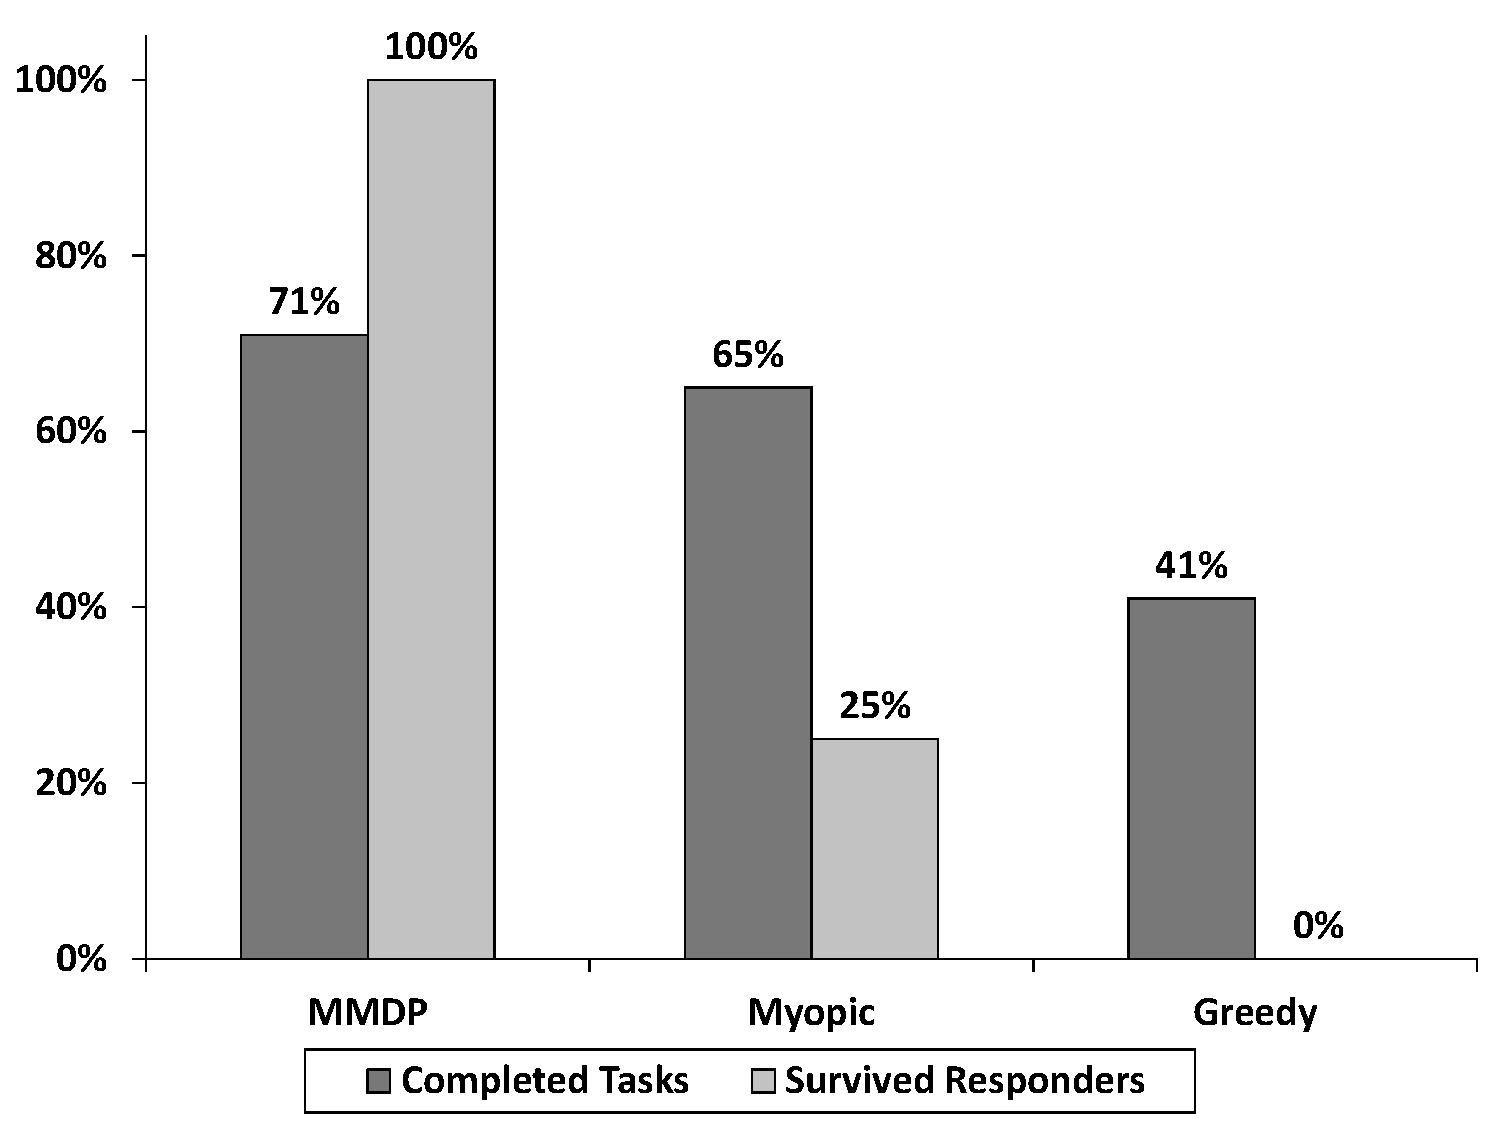
\includegraphics[width=0.8\linewidth]{simulation}
%  \caption{Experimental results for the MMDP, myopic, greedy
%  algorithms in simulation.}
%  \label{fig:simulation}
%\end{figure}


\noindent Before deploying our solution (as part of $PA$) to advise
human responders, it is important  to test its performance to
ensure it can return efficient solutions on simulations of the
real-world problem. Given there is no extant solution that
takes into account uncertainty in team coordination for emergency
response, we compare our algorithm with a greedy and a
myopic method to evaluate the benefits of coordination and
lookahead. For each method, we use our path planning algorithm to
compute the path for each responder. In the greedy method, the responders
are uncoordinated and select the closest tasks they can do. In
the myopic method, the responders are coordinated to select the
tasks but have no lookahead for the future tasks (Line 8 in
Algorithm~\ref{alg:taskplanning}). Table~\ref{tab:simulation} shows
the results for a problem with 17 tasks and 8 responders on a
50$\times$55 grid. As can be seen, our MMDP algorithm 
completes more tasks than the myopic and greedy methods (see Table
\ref{tab:simulation}). More importantly, our algorithm guarantees
the safety of the responders, while in the myopic method  only 25\%
of the responders survive and in the greedy method all responders
are killed by the radioactive cloud. More extensive evaluations are
beyond the scope of this paper as our focus here is on the use of
the algorithm in a field deployment to test how humans take up
advice computed by the planning agent $PA$.
\begin{table}[htbp]
  \centering
  \caption{Experimental results for the MMDP, myopic, greedy
  algorithms in simulation.}
  \begin{tabular}{l|c|c|c}
   & MMDP & Myopic & Greedy \\
  \hline
  No. of completed tasks & 71\% & 65\% & 41\% \\
  \hline
  No. responders alive at the end & 100\% & 25\% & 0\% \\
  \end{tabular}
  \label{tab:simulation}\vspace{-3mm}
\end{table}


\end{document}
